\section{Durchführung}
\label{sec:Durchführung}

Es werden für die verschiedenen Druckbereiche zwei unterschiedliche Apparaturen verwendet. \\
Im niedrigen Bereich von $p \leqslant 1\:bar$ wird mit dem folgenden Aufbau gemessen

\begin{figure}[H]
    \centering
    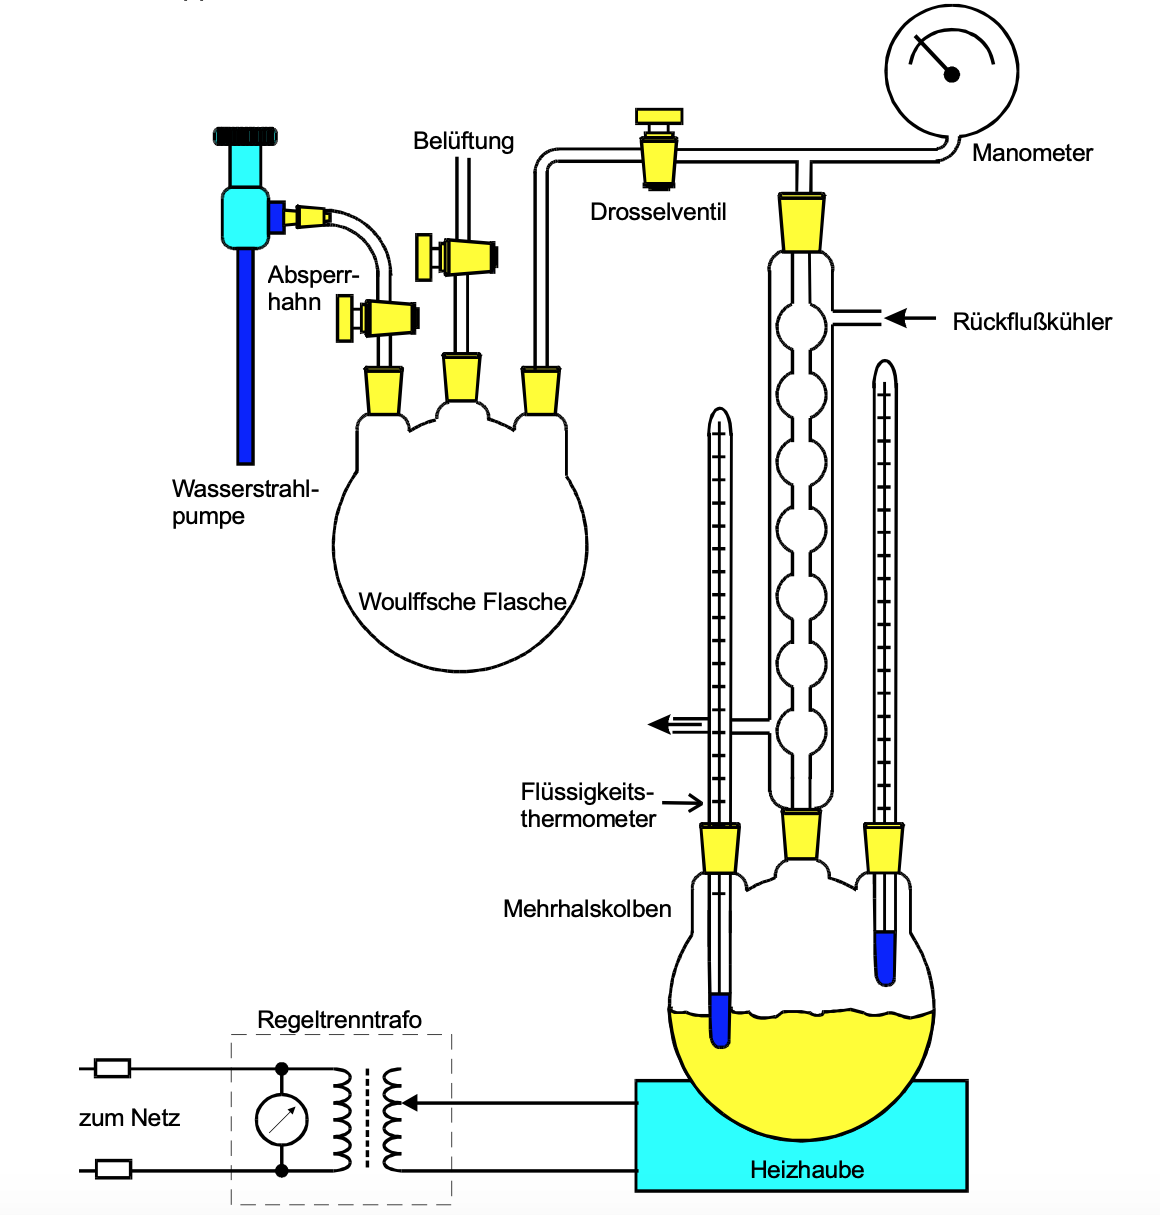
\includegraphics[scale=0.5]{content/v203_abb1.png}
    \caption{Die für $p \leqslant 1\:bar$ verwendete Apparatur. \cite{sample}}
    \label{abb:niedrigdruck}
\end{figure}
Zu Beginn wird mittels Wasserstrahlpumpe evakuiert, bis der niedrigste mögliche Druck von $38\:mbar$ erreicht ist.\\ % noch benennen

Bei jedem Anstieg der Temperatur um $2°C$ wird der Druck vom digitalen Manometer abgelesen und notiert.\\


Für höhere Druckbereiche ($p \geqslant 1\:bar$) wird die Messung mit folgendem Gerät durchgeführt

\begin{figure}[H]
    \centering
    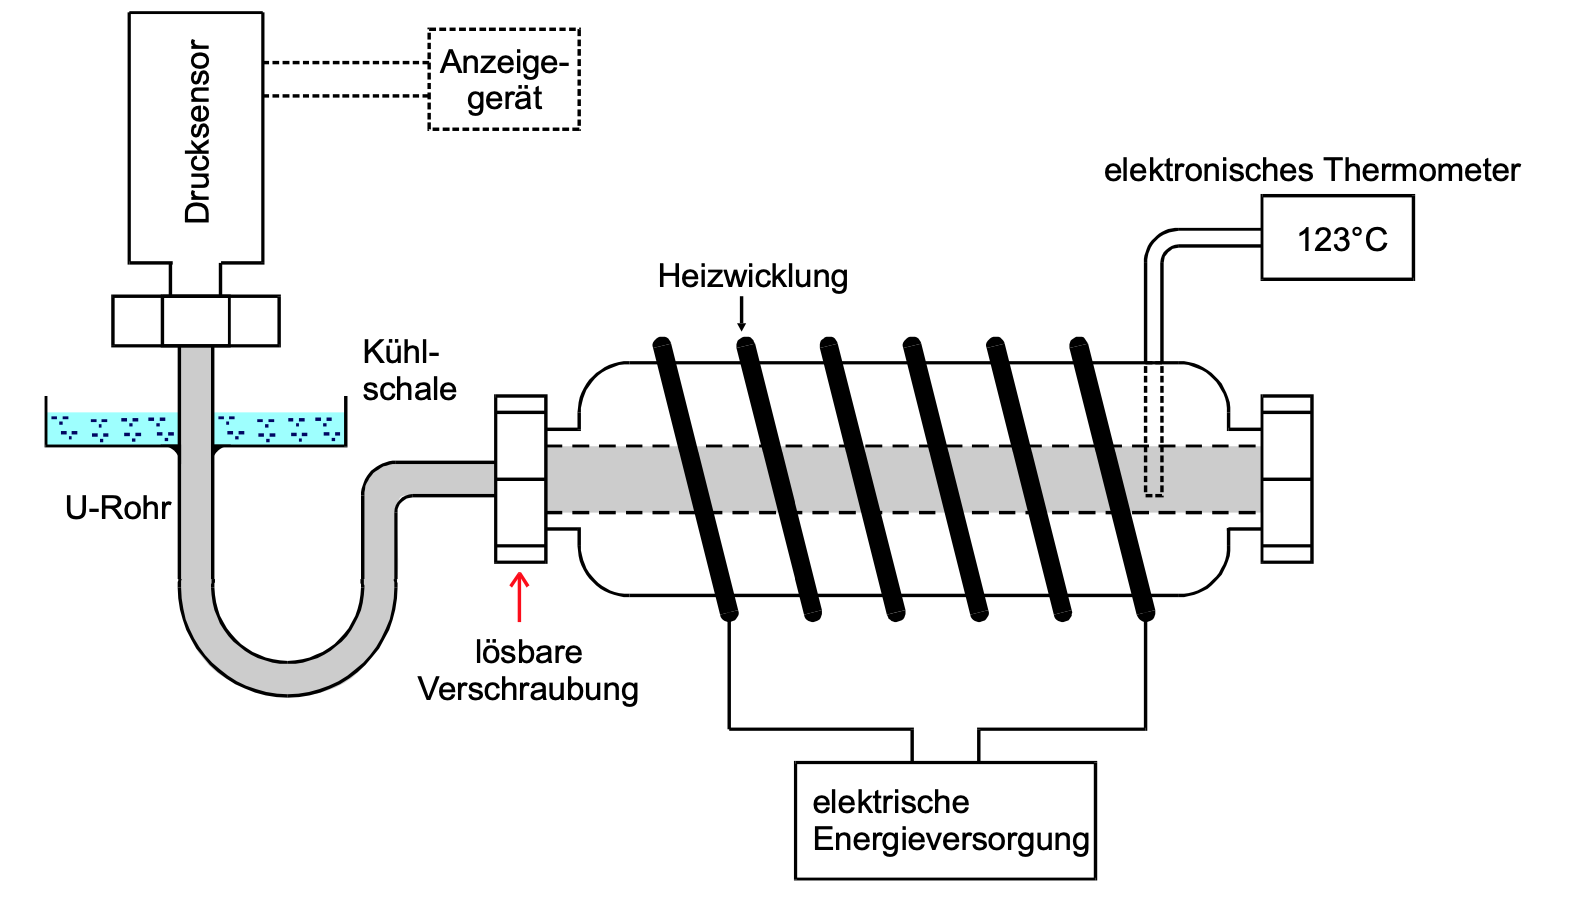
\includegraphics[scale=0.5]{content/v203_abb2.png}
    \caption{Die für $p \geqslant 1\:bar$ verwendete Apparatur. \cite{sample}}
    \label{abb:hoherdruck}
\end{figure}

Bei jedem vollen Druck-Wert von $1$ bis $15\:bar$ über dem Atmosphärendruck wird die Temperatur in $°C$ vom Thermometer abgelesen.\\
Anders, als in der Abbildung dargestellt, wird ein analoges Theromometer verwendet.\\